\documentclass[aspectratio=43,display]{beamer}
\mode<presentation>
{
  \usetheme{Montpellier}      % or try Darmstadt, Madrid, Warsaw, ...
  \usecolortheme{dove} % or try albatross, beaver, crane, ...
  \usefonttheme{default}  % or try serif, structurebold, ...
  \setbeamertemplate{navigation symbols}{}
  \setbeamertemplate{caption}[numbered]
} 

\usepackage[english,russian]{babel}
\usepackage[utf8x]{inputenc}
\usepackage{siunitx}
\usepackage{enumerate}
\usepackage{hyperref}
\usepackage{eso-pic}
\usepackage{mathbbol}
\usepackage{bm}
\usepackage{nccmath}
\graphicspath{{pics}}
\hypersetup{
	bookmarksopen=false,
	pdfpagemode=UseNone,
	%pdfpagemode=FullScreen,   %% Enable to have Adobe Reader query for fullscreen mode
	pdfauthor={Detlev Conrad Mielczarek} %% Enter the apppropriate author in here
}

\newcommand\AtPagemyUpperLeft[1]{\AtPageLowerLeft{%
		\put(\LenToUnit{0.90\paperwidth},\LenToUnit{0.89\paperheight}){#1}}}
	\AddToShipoutPictureFG{
	\AtPagemyUpperLeft{{
\includegraphics[width=0.8cm,keepaspectratio]{BMSTU_logo.png}}}
}%

\title[]{Использование кластерного блока чувствительных элементов для поиска и устранения cycle-slip в интегрированном спутниковом навигационном приемнике}
%% Author with both abbreviation and affiliation
\author[FH, TE, ST]{Новичков А.Р.\inst{1} \and Гончаров И.К.\inst{1}\and Егорушкин А.Ю.\inst{1}}
\institute[BMSTU]{\inst{1}Московский Государственный Технический Университет
	имени Н.Э. Баумана\\МГТУ им. Н.Э. Баумана}
\date[NMC 2021]{International Workshop Navigation and Motion Control, 2021}

\begin{document}

\begin{frame}
  \titlepage
\end{frame}

% Uncomment these lines for an automatically generated outline.
%\begin{frame}{Outline}
% \tableofcontents
%\end{frame}

\section{Введение}
\begin{frame}{Введение}
\begin{itemize}
  \item Кластерный блок чувствительных элементов
  \item Оценка погрешностей кластерного инерциального блока
  \item Оценка выходных погрешностей БИНС на базе кластерного инерциального блока
  \item Схема интеграции ИНС/ГНСС
  \item Дальнейшие планы
\end{itemize}
\vskip 1cm
%\begin{block}{Examples}
%Some examples of commonly used commands and features are included, to help you get started.
%\end{block}
\end{frame}


\section{Кластерный блок чувствительных элементов}
%\subsection{Tables and Figures}
\begin{frame}{Кластерный блок чувствительных элементов}
% Картинка кластера
\begin{figure}
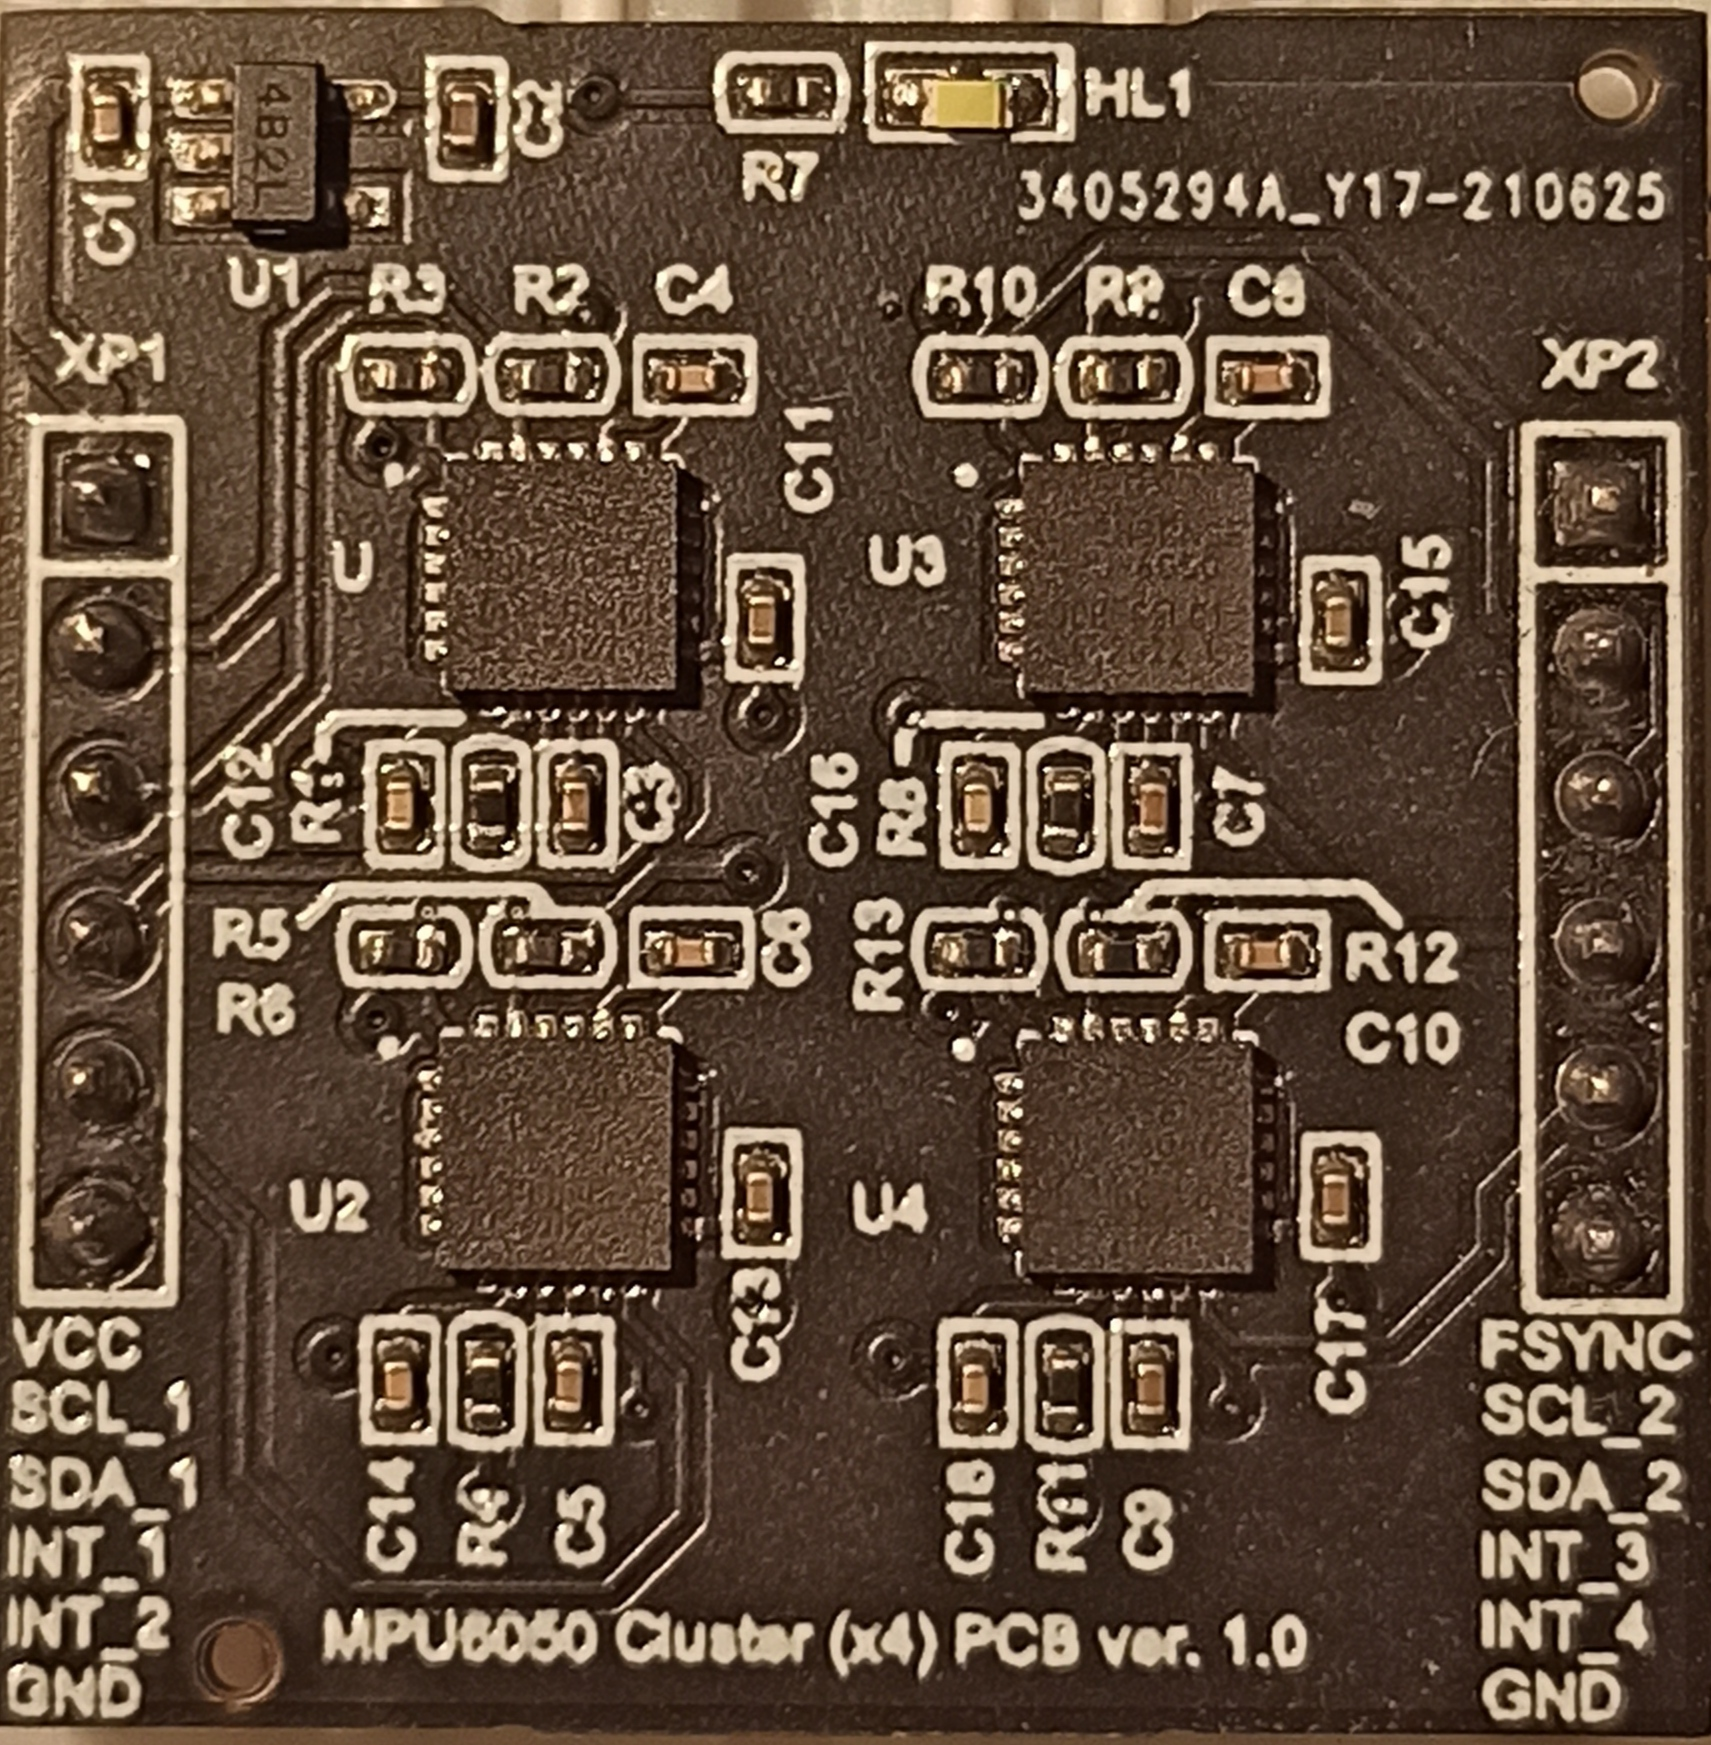
\includegraphics[width=0.45\linewidth]{cluster_pcb.jpg}
\caption{\label{fig:cluster_pcb} Печатная плата кластерного БЧЭ}
\end{figure}
\end{frame}


\subsection{Погрешности чувствительных элементов}
\begin{frame}{Остаточная погрешность чувствительных элементов}
\begin{figure}
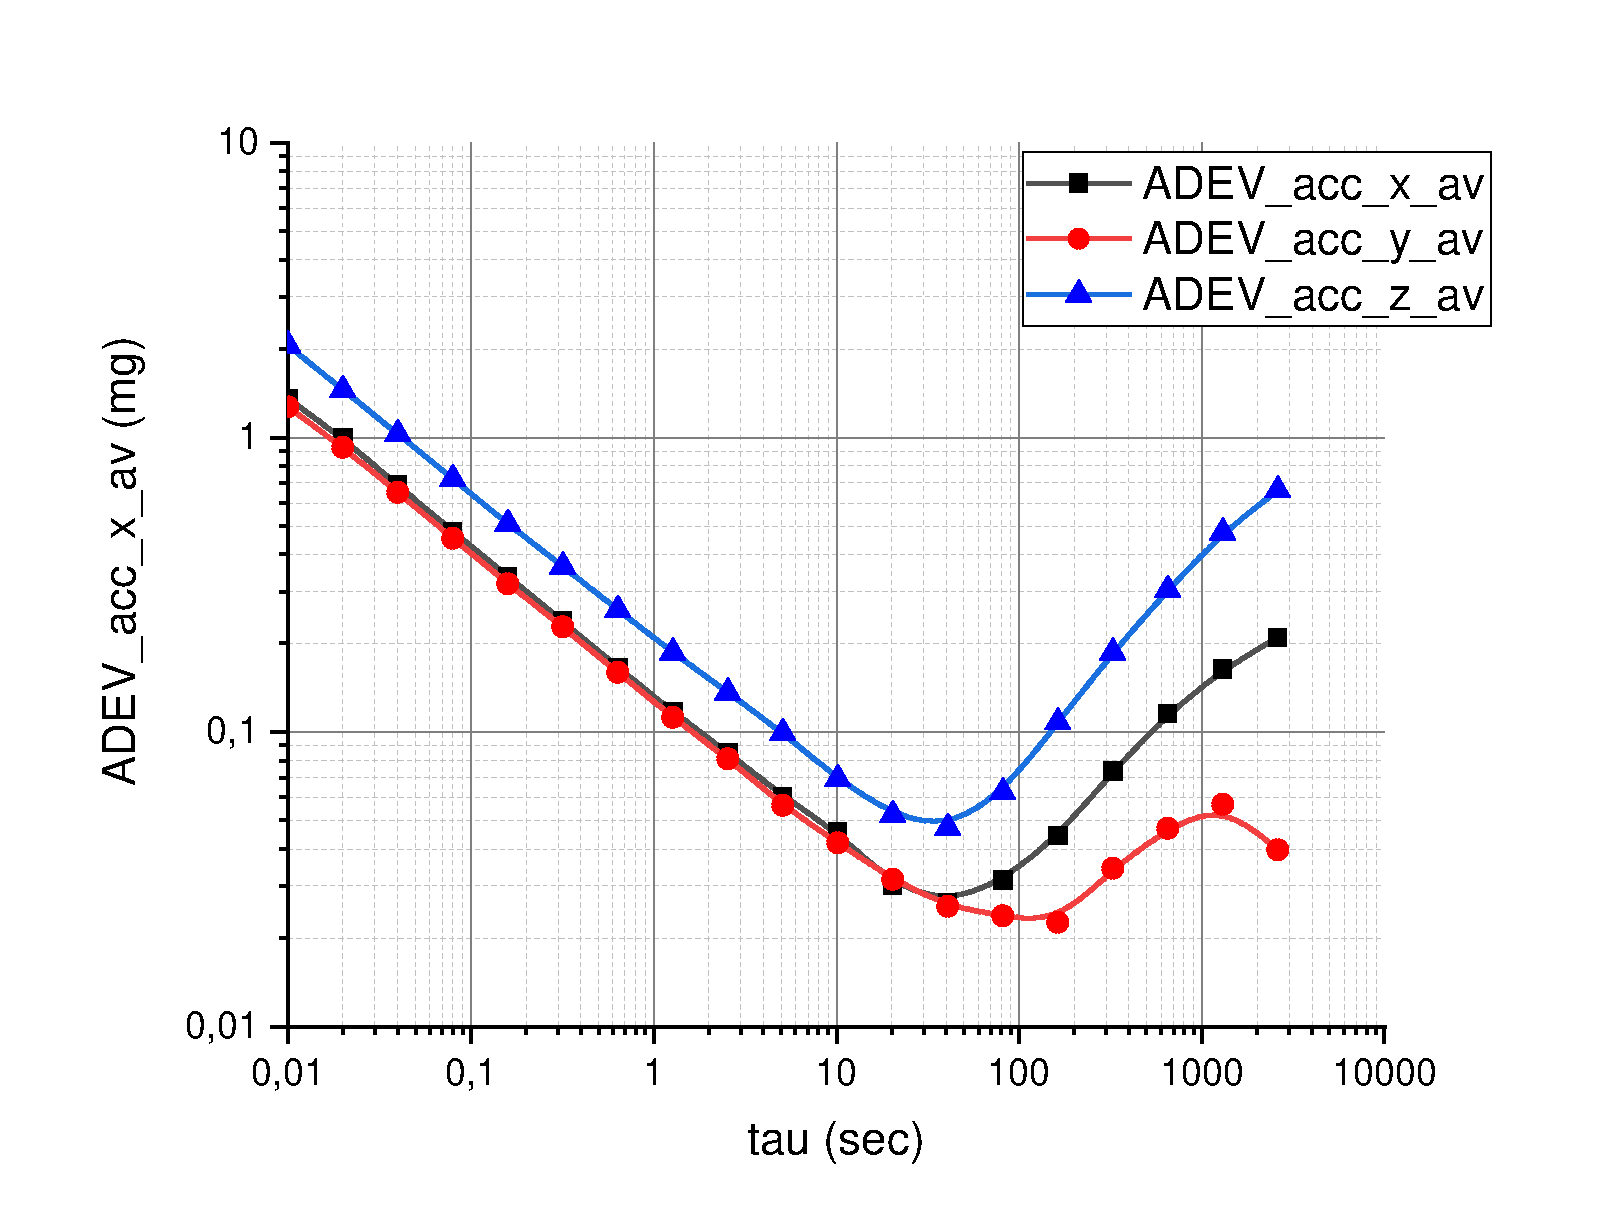
\includegraphics[width=0.7\linewidth]{acc_av_adev.pdf}
\caption{\label{fig:mpr_1} Девиации Аллана для акселерометров}
\end{figure}	
\end{frame}


\begin{frame}{Остаточная погрешность чувствительных элементов}
\begin{figure}
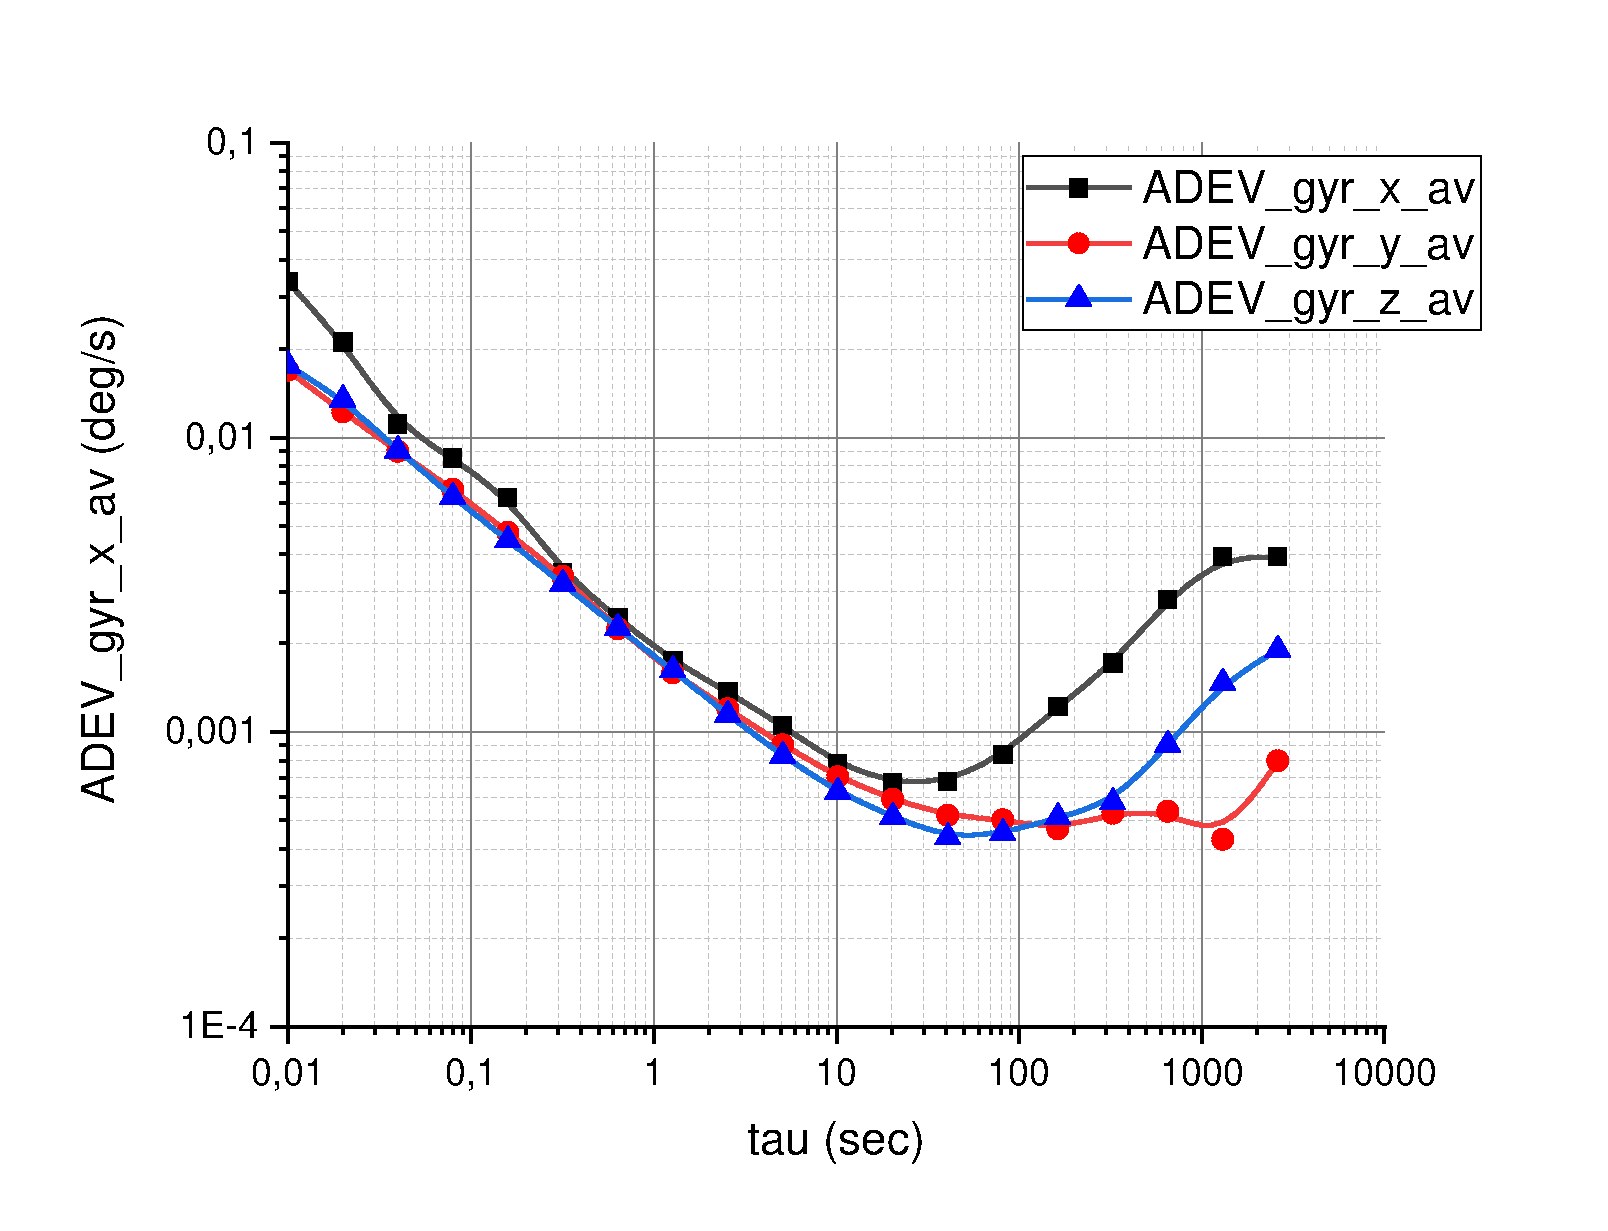
\includegraphics[width=0.7\linewidth]{gyr_av_adev.pdf}
\caption{\label{fig:mpr_2} Девиации Аллана для гироскопов}
\end{figure}
\end{frame}


\section{Выходные погрешности ИНС}
\subsection{Уравнения выходных ошибок ИНС}
\begin{frame}{Выходные погрешности БИНС}


\begin{equation}
	\label{eq:V_e}
	\small
	\begin{gathered}
		\delta V_e(t) = - \varPhi_y(0) R \sin \nu t + \delta V_x(0) \cos \nu t - \xi_y R (1 - \cos \nu t) + \\
		\frac{\sin \nu t}{ \nu } B_x(0)
	\end{gathered}
\end{equation}


\begin{equation}
	\label{eq:V_n}
	\small
	\begin{gathered}
		\delta V_n(t) = - \varPhi_x(0) R \sin \nu t + \delta V_y(0) \cos \nu t + \xi_x R (1 - \cos \nu t) + \\
		\frac{\sin \nu t}{ \nu } B_y(0)
	\end{gathered}
\end{equation}


\begin{equation}
	\label{eq:lambda}
	\small
	\begin{gathered}
		\lambda (t) = \int \frac{\delta V_e(t)}{R \cos \phi} dt
	\end{gathered}
\end{equation}

\begin{equation}
	\label{eq:phi}
	\small
	\begin{gathered}
		\phi (t) = \int \frac{\delta V_n(t)}{R \cos \phi} dt
	\end{gathered}
\end{equation}	

\vspace{0.15cm}
где { \small $ \nu = \sqrt{ \frac{g}{R} } $ } - шулеровская частота колебания;


{\small $ B_x(0), B_y(0) $} - смещения нулей акселерометра;


{\small $ \xi_x, \xi_y, \xi_z $} - дрейф гироскопа;
\end{frame}


\subsection{Результат моделирования}
\begin{frame}{Погрешность в определении координат}
	\begin{figure}
		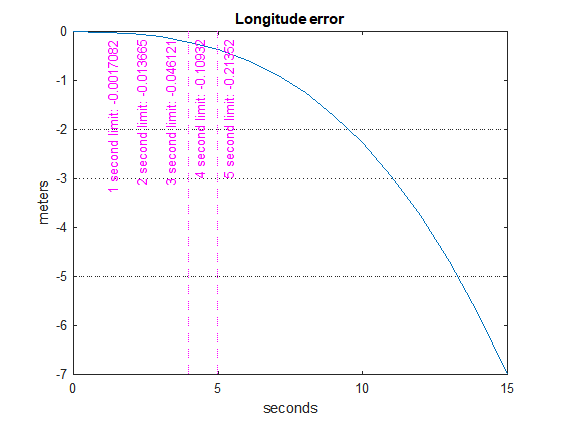
\includegraphics[width=0.7\linewidth]{longitudeError.png}
		\caption{График нарастания ошибки в определении долготы места}
		\label{fig:long_error}
	\end{figure}
\end{frame}


\begin{frame}{Погрешность в определении координат}
	\begin{figure}
		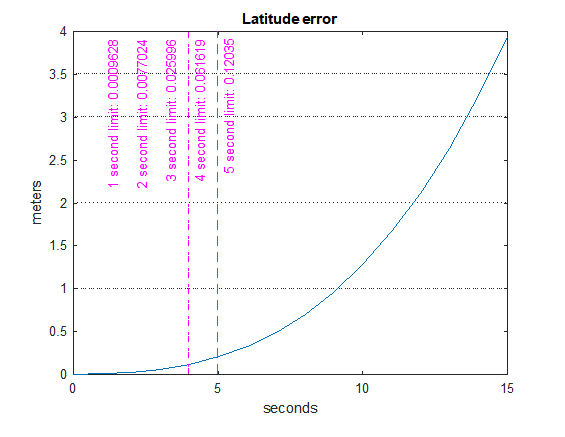
\includegraphics[width=0.7\linewidth]{latitudeError.png}
		\caption{График нарастания ошибки в определении широты места}
		\label{fig:lat_error}
	\end{figure}
\end{frame}


\section{Интеграция ИНС/СНС}
\subsection{Тесная интеграция ИНС/СНС}
\begin{frame}{Схема интеграции ИНС/ГНСС}
	\begin{figure}
		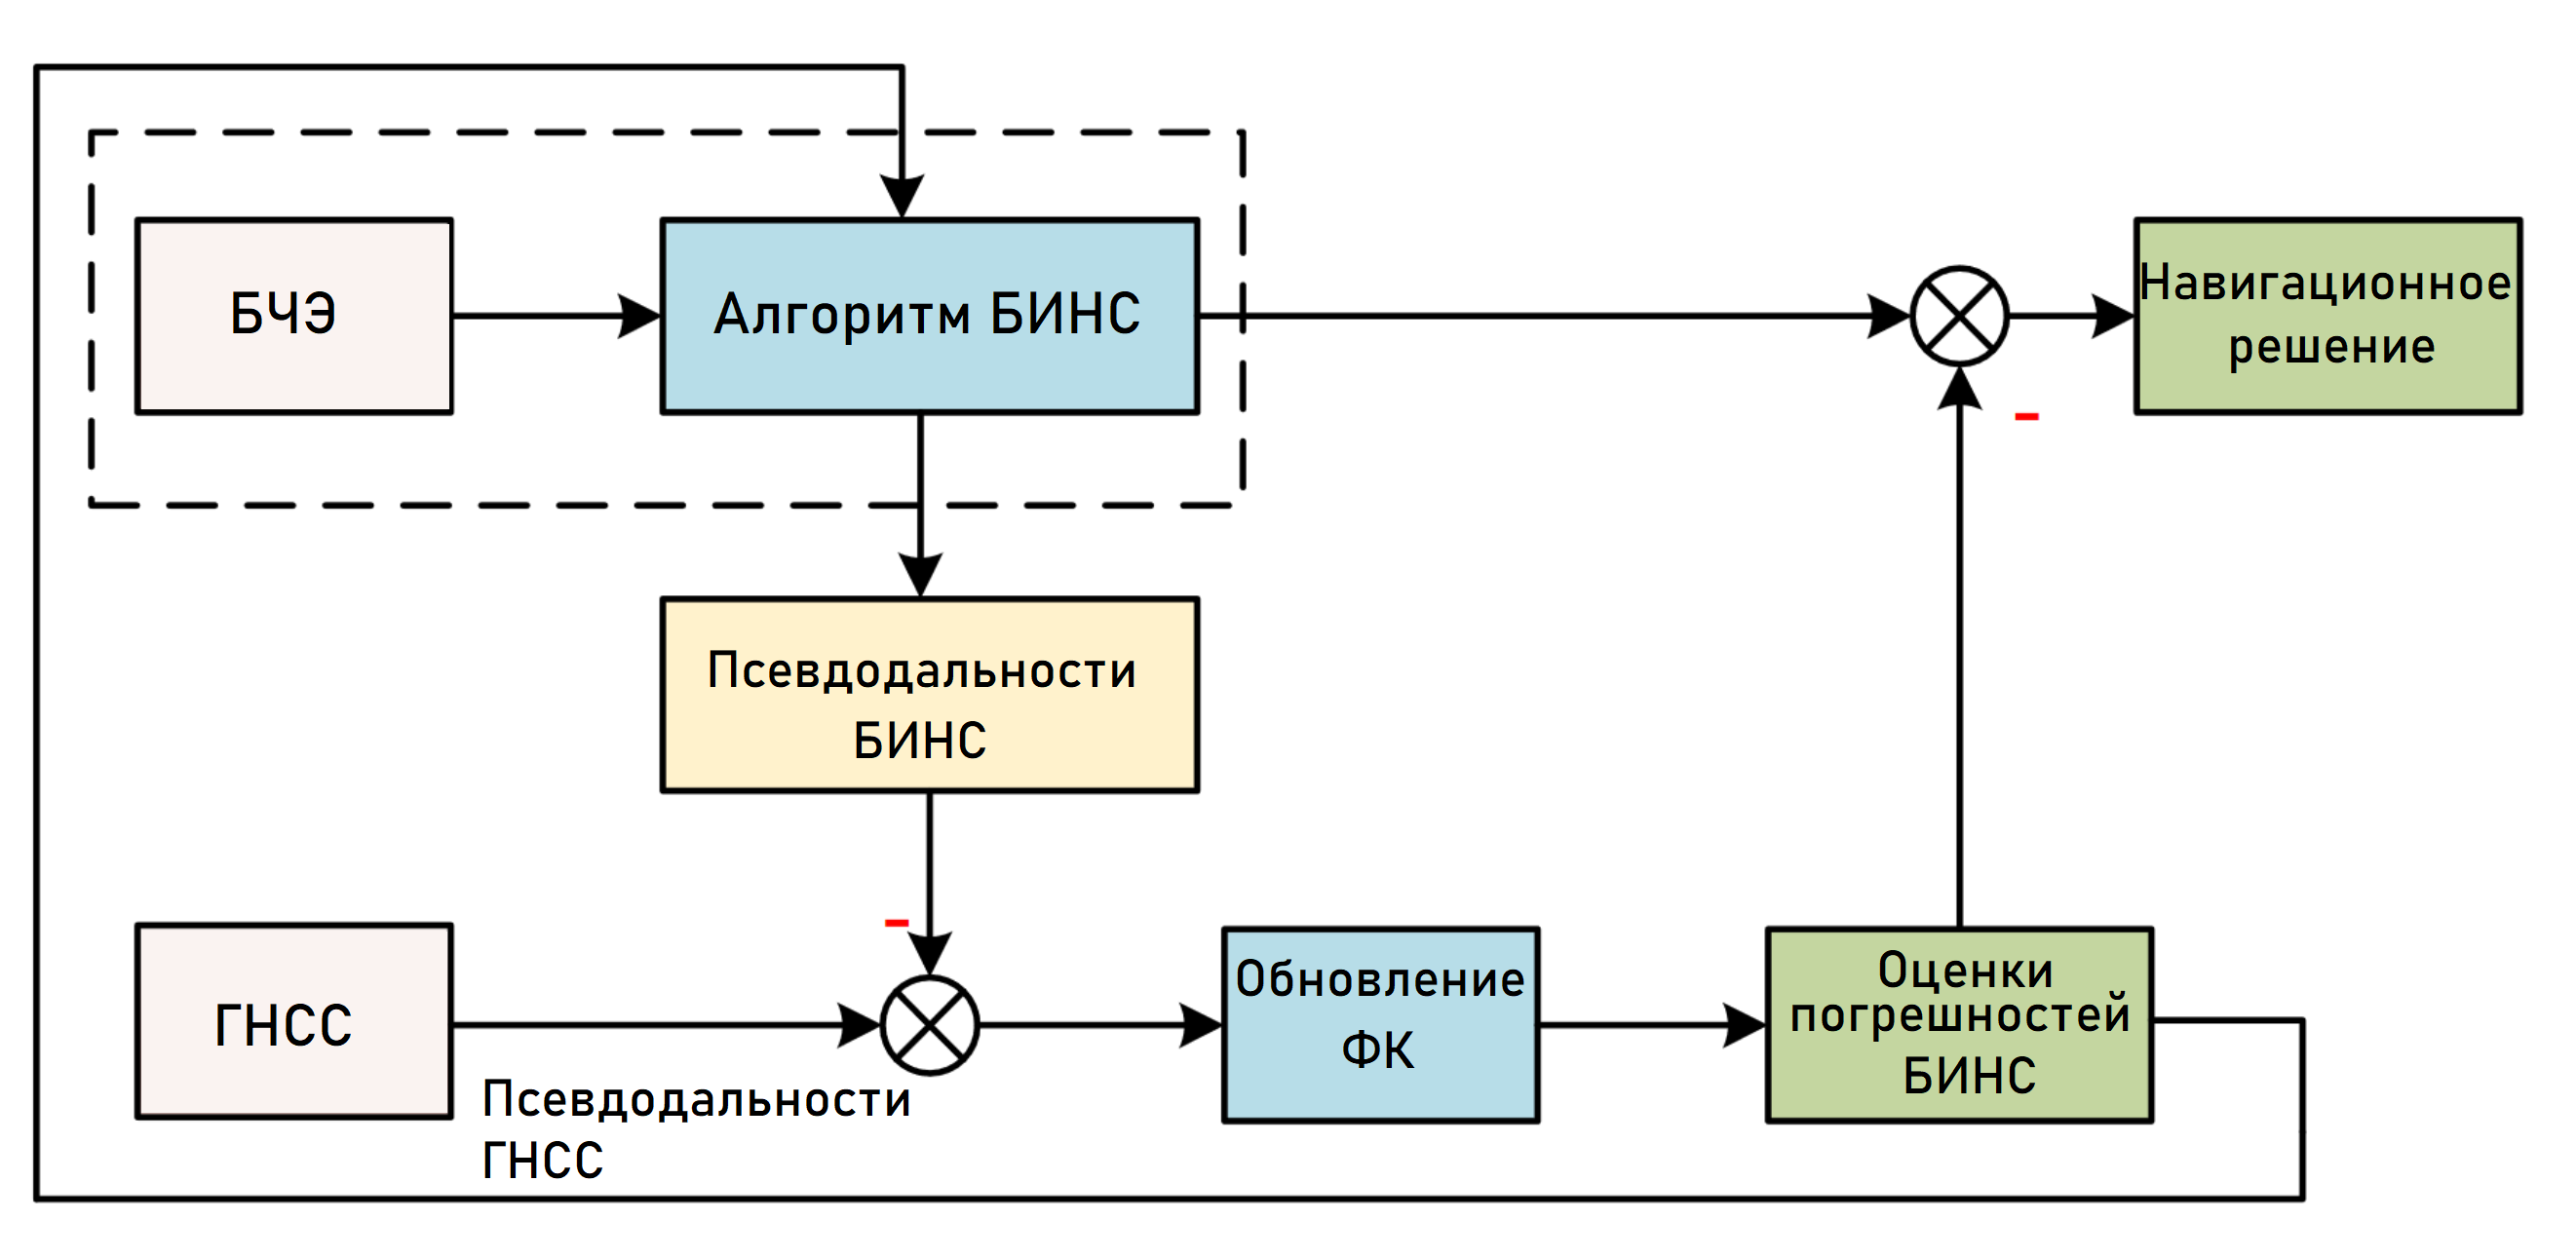
\includegraphics[width=1.0\linewidth]{integration.png}
		\caption{\label{fig:cluster_pcb} Схема интеграции ИНС/ГНСС}
	\end{figure}
\end{frame}


\begin{frame}{Алгоритм БИНС}

\begin{fleqn}
\begin{equation} \label{eq:tr_mat}
	\begin{gathered}
	\begin{split}
		& \bm C_b^e(+) = \bm C_b^e(-) \bm C_{b+}^{b-} - \bm \Omega_e \bm C_b^e(-) \tau_{ins} \\
		&  \bm C_{b+}^{b-} = I_3 + \sin \alpha (\alpha \times) / \alpha + (1 - \cos \alpha )(\bm \alpha \times)^2 / \alpha^2 \\ 
		& \bm \alpha =  \bm \omega\tau_{ins}, \alpha = \parallel \bm \alpha \parallel
	\end{split}
	\end{gathered}
\end{equation}

\begin{equation}
	\label{eq:vel}
	\begin{split}
			& \bm v_{ins} (+) = \bm v_{ins}(-) + (\bm f_e + \bm g (\bm r_{ins}(-) - 2 \bm \Omega_e \bm v_{ins} (-) ) )  \tau_{ins} \\
			& \bm f_{ins} = (\bm C_b^e(-) \bm C_b^e(+)) \bm f / 2
	\end{split}
\end{equation}	

\begin{equation}
	\label{eq:vel}
		\bm r_{ins}(+) = \bm r_{ins}(-) + (\bm v_{ins}(-) + \bm v_{ins}(+)) \tau_{ins}/2
\end{equation}
\end{fleqn}
\end{frame}


\begin{frame}{Модель измерений интегрированной системы}
		
	Вектор состояния для случая тесной интеграции: 
	
	\begin{equation} \label{eq:tr_mat}
		x = (\delta \psi_{ins} ^ T, \delta r_{ins} ^ T, \delta v_{ins} ^ T, 
		b_{a} ^ T, b_{g} ^ T) ^ T
	\end{equation}

\vspace{0.5cm}

\begin{fleqn}
	\begin{equation} \label{eq:tr_mat}
		\begin{split} 
				& \hat{C_b^e} = (I_3 - \delta \hat{\psi_{ins}} \times)C_b^e \\
				& \hat{r_{ins/gps}} = r_{ins} + \delta \hat{r_{ins}} + \hat{C_b^e}l_{r} \\ 
				& \hat{v}_{ins/gps} = v_{ins} + \delta \hat{v}_{ins} + \hat{C_b^e} (\omega \times l_r) + \Omega_e \hat{C_b^e} l_r \\ 
				& \rho_r^i = \parallel \hat{r_{ins/gps}} - r^i \parallel, 
				\parallel \hat{v_{ins/gps}} - v^i \parallel  
		\end{split}
	\end{equation}
\end{fleqn}

\end{frame}


\begin{frame}{Модель измерений интегрированной системы}
	
	\begin{equation}
		\label{eq:ins_19}
		h(\hat{x}) = (h_p(\hat{x})^T, h_{\dot{p}}(\hat{x})^T)^T
	\end{equation}

\vspace{0.5cm}

	\begin{equation*}
		h_p(\hat{x}) = 
		\begin{pmatrix}
			\rho_r^{12} - cdT^{12} \\
			\rho_r^{13} - cdT^{13} \\
			\vdots \\ 
			\rho_r^{1m} - cdT^{1m} \\
		\end{pmatrix}
		,
		h_{\dot{p}}(\hat{x}) = 
		\begin{pmatrix}
			\dot{\rho}_r^{12} - cd\dot{T}^{12} \\
			\dot{\rho}_r^{13} - cd\dot{T}^{13} \\
			\vdots \\ 
			\dot{\rho}_r^{1m} - cd\dot{T}^{1m} \\
		\end{pmatrix}
	\end{equation*}

\vspace{0.5cm}

	\begin{equation}
		\label{eq:ins_20}
		H(\hat{x}) = \frac{\partial h(x)}{\partial x}\bigg{|}_{x=\hat{x}} = 
		\begin{pmatrix}
			0 & -DE & 0 & 0 & 0 \\ 
			0 & 0 & -DE & 0 & 0
		\end{pmatrix}
	\end{equation}

\end{frame}

\begin{frame}{Матрица перехода}
	\begin{equation}
		\label{eq:ins_21}
		F_k^{k+1} = 
		\begin{pmatrix}
			I_3 - \Omega_e \tau_r & 0 & 0 & 0 & \hat{C}_b^e \tau_r\\
			0 & I_3 & I_3 \tau_r & 0 & 0 \\
			-(\hat{C}_b^e f \times) \tau_r & 0 & I_3 - \Omega_e \tau_r & \hat{C}_b^e \tau_r & 0\\
			0 & 0 & 0 & I_3 & 0 \\
			0 & 0 & 0 & 0 & I_3 \\
		\end{pmatrix}
	\end{equation}
\end{frame}


\section{Схема детекции сycle-slip с использованием БИНС}
\begin{frame}
	
\vspace{0.25 cm}
	
	\begin{equation}
		\label{eq:ins_22}
		\begin{split}
			& \bm { \hat{r}_{r,k+1}(-) = \hat{r}_{r,k}(+) + (\hat{\nu}_{ins/gps,k+1} + \hat{\nu}_{ins/gps,k})\tau_r/2 } \\
			& \bm{ \hat{\nu}_{r,k+1}(-) = \hat{\nu}_{ins/gps,k+1} }\\
			& \bm{P}_{k+1} = \bm{F}_k^{k+1} \bm{P}_k(+) \bm{F}_k^{k+1^T} + \bm{Q}_k^{k+1}
		\end{split}
	\end{equation}
	
	\begin{equation*}
		\label{eq:F_k}
		\bm{F}_k^{k+1} = 
		\begin{pmatrix}
			\bm{I}_3 & & & \\
			& 0 & & \\
			& & \bm{I}_{m-1} & \\
			& & & \bm{I}_{m-1}
		\end{pmatrix}
	\end{equation*}
	
	\begin{equation*}
		\label{eq:Q_k}
		\bm{Q}_k^{k+1} = 
		\begin{pmatrix}
			\bm{P}_{\nu-ins/gps,k+1} \tau_r & & & \\
			& \bm{P}_{\nu-ins/gps,k+1}  & & \\
			& & 0 & \\
			& & & 0
		\end{pmatrix}
	\end{equation*}	
\end{frame}


\begin{fleqn}
\begin{frame}
	
	Невязки с учётом динамики объекта, оцененной при помощи БИНС:
	\begin{equation}
		\label{eq:ins_23.1}
			\nu = y_k - h(\hat{x}_k(-))			
	\end{equation}
	
	Ковариационная матрица априорной ошибки оценивания: 
	\begin{equation}
		\label{eq:ins_23.2}
		\begin{split}
			Q_{\nu} = H(\hat{x}_k(-))P_k(-)H(\hat{x}_k(-))^T + R_k
		\end{split}
	\end{equation}
	
	Критерий детектирования cycle-slip фазовых измерений: 
	\begin{equation}
		\label{eq:ins_24}
		\nu_i^2 > nq_{i, \nu}
	\end{equation}
\end{frame}
\end{fleqn}

\end{document}